\documentclass{standalone}
\usepackage{tikz}
\usepackage{caption}
\usepackage{subcaption}
\usepackage{helvet}
\usepackage{adjustbox}
\renewcommand{\familydefault}{\sfdefault}
\usetikzlibrary{
  positioning, calc, shapes.geometric, shapes.multipart, 
	shapes, arrows.meta, arrows, 
	decorations.markings, external, trees}

% Arrow style:
\tikzset{
    Arrow/.style = {
        thick, 
        decoration={
            markings,
            mark=at position 1 with {
                \arrow[thick, #1]{latex}
                }
            }, 
        shorten >= 3pt, 
        preaction = {decorate}
    },
    Arrow/.default={black}
}
% Text node
\tikzset{
Node/.style={
  text width=1cm,
  align=center,
  }
}
% Colors
\definecolor{aFill}{HTML}{2980b9}
\definecolor{tFill}{HTML}{67A0C6}
\definecolor{yFill}{HTML}{3B4247}
\definecolor{uFill}{HTML}{bdc3c7}
\definecolor{uColor}{HTML}{fc5c65}
\begin{document}
\begin{adjustbox}{width=20cm, height=12cm, keepaspectratio}
  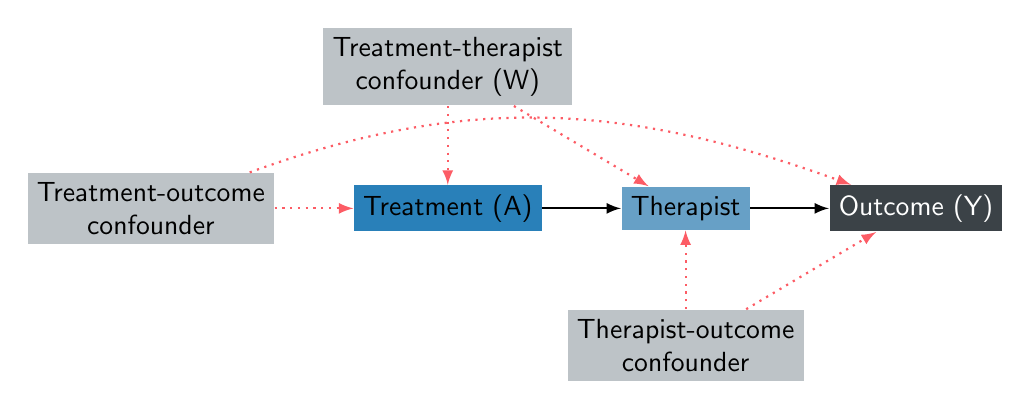
\begin{tikzpicture}
    \node [fill=uFill, align=center](U) {Therapist-outcome\\confounder};
    \node [fill=tFill, above=1cm of U](T) {Therapist};
    \node [fill=aFill, left=of T] (A) {Treatment (A)};
    \node [fill=uFill, left=of A, align=center](U1) {Treatment-outcome\\confounder};
    \node [fill=uFill, above=of A, align=center](W) {Treatment-therapist\\confounder (W)};
    \node [fill=yFill, text=white, right=of T] (Y) {Outcome (Y)};
    \draw [Arrow=uColor, color=uColor, dotted] (U) to (T);
    \draw [Arrow=uColor, color=uColor, dotted] (U) to (Y);
    \draw [Arrow=uColor, color=uColor, dotted] (W) to (A);
    \draw [Arrow=uColor, color=uColor, dotted] (W) to (T);
    \draw [Arrow=uColor, color=uColor, dotted] (U1) to (A);
    \draw [Arrow=uColor, color=uColor, dotted] (U1) to [in=160, out=20] (Y);
    \draw [Arrow] (A) to (T);
    \draw [Arrow] (T) to (Y);
  \end{tikzpicture}
\end{adjustbox}
\end{document}